\subsection{The Selection of Cities}
Section \ref{sec:eceexperiences} shows that the childcare systems within and outside Reggio Emilia share the Reggio Approach components to varying degrees. Because other childcare options may be similar to the Reggio Approach to some extent and may have their own high-quality components, it is difficult to evaluate the clean effects of the Reggio Approach. Our survey data collection is designed to evaluate the impact of the Reggio Approach relative to other programs that share similar components. Note that our comparison is not to determine whether Reggio is of higher or lower quality relative to other programs but to understand how the programs are different across school types, cities, and over time. 

We collect data on the individuals in Reggio Emilia, Parma, and Padova. Parma and Padova
have been chosen in addition to Reggio Emilia to represent appropriate controls: they are close enough to
Reggio Emilia in terms of size, geographic, demographic, and socio-economic
structure, but they did not experience its unique approach to early
childhood education.\footnote{%
Other Italian cities were taken into consideration, notably Brescia,
Livorno, Modena, Perugia, Piacenza, Prato, and Ravenna. Parma and Padova
were the two cities that best fulfilled our comparability and sample
requirements.} For example, Reggio Emilia has a population of roughly
173,000, Parma of 188,000, and Padova of 210,000 in 2013.\footnote{%
The population size in December 2013 was 172,525 in Reggio Emilia, 187,938
in Parma, and 209,678 in Padova. Source: ISTAT, %
\url{http://www.demo.istat.it/}} Also their economic resources are
comparable: Reggio Emilia has an average per-capita income of 25,226 euros,
Parma of 28,437, and Padova of 29,915 in 2011.\footnote{%
Source: Finance Minister, taxable income for 2011.} 
%See \url{http://www.comuni-italiani.it/statistiche/redditir2011.html}
Even more importantly, these three cities face analogous fertility dynamics
and, consequently, potential demand for child-care services. The three
cities had a very similar number of births from both Italians and immigrants
in the past decade. Parma is a neighboring city 30 km to the west of Reggio
Emilia, it belongs to the same administrative region of Emilia-Romagna, and
shares with Reggio a common background that forged the city's political and
economic system, and shaped its culture and social capital; yet Parma has
witnessed a different approach to public investment in early childhood
education. On the contrary, Padova lies 150 km away from Reggio Emilia, in
the richer north-eastern region of Veneto, and was more influenced by the
history and culture of Venice. Yet, Padova, just as Reggio Emilia, is a middle-size
Italian city with a thriving migrant population, facing similar political
and economic issues, with a different social background but similar
resources which can be devoted to early childhood education.

Statistics on preschool enrollment is different across three cities, which is presented in Figure \ref{fig:enrollment}. Note that enrollment data is not available for Parma except for the year 2010. It is shown that Reggio Emilia and Padova observed the increase in preschool enrollment; from 1990s on, almost all children of age 3-5 are enrolled in preschool. The figures also show that the percentage of enrollment in municipal preschools increased during the 1970s and the 1980s in Reggio Emilia and Padova, but decreased after the 1990s in Reggio Emilia. The percentage enrolled in state preschools increased over time in both Reggio Emilia and Padova. In contrast, the percentage enrolled in private preschools decreased over time in Reggio Emilia and Padova. For Parma, the enrollment statistics in 2010 are similar to those of Reggio Emilia. 
 
\begin{figure}[H] \label{fig:enrollment}
      \centering
        \begin{subfigure}[t]{0.49\textwidth}
          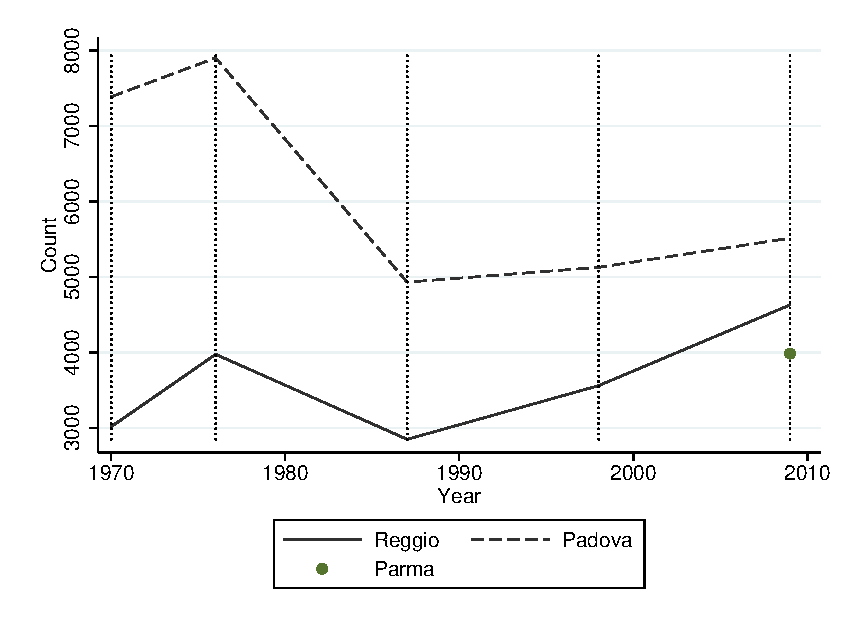
\includegraphics[width=\textwidth]{../../output/image/enroll_num_graph.eps}       
\caption{Num. of Children Enrolled in Preschool}        
        \end{subfigure}
        \begin{subfigure}[t]{0.49\textwidth}
          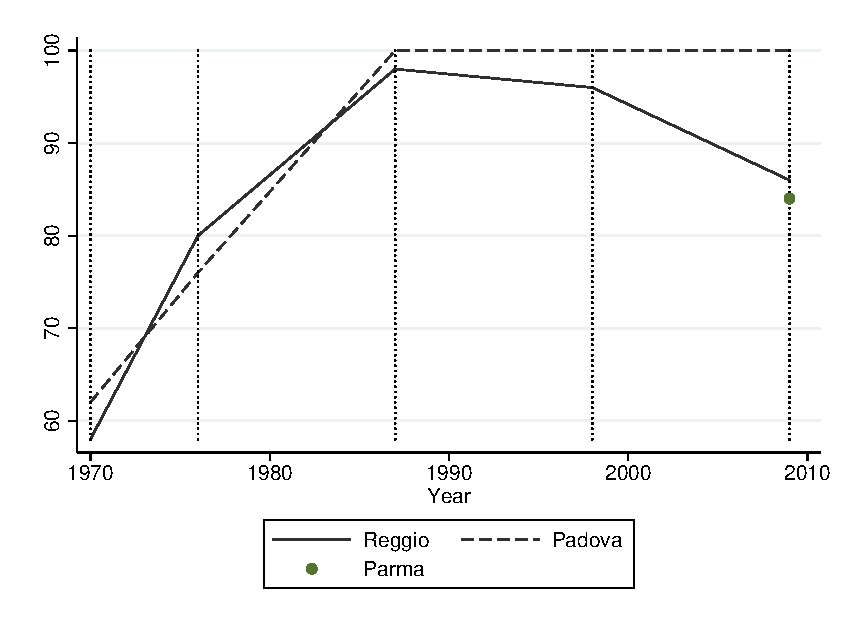
\includegraphics[width=\textwidth]{../../output/image/enroll_per_graph.eps}       
 \caption{Percent. of Ages 3-5 Enrolled}        
        \end{subfigure}
        \begin{subfigure}[t]{0.49\textwidth}
          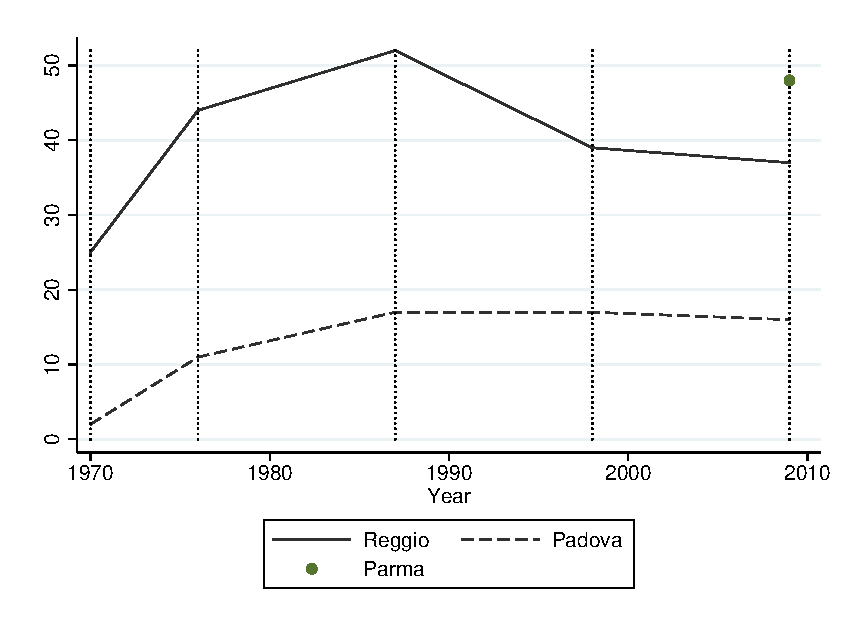
\includegraphics[width=\textwidth]{../../output/image/enroll_per_muni_graph.eps} 
        \caption{Percent. of Enrollment in Municipal Preschool}        
        \end{subfigure}
        \begin{subfigure}[t]{0.49\textwidth}
          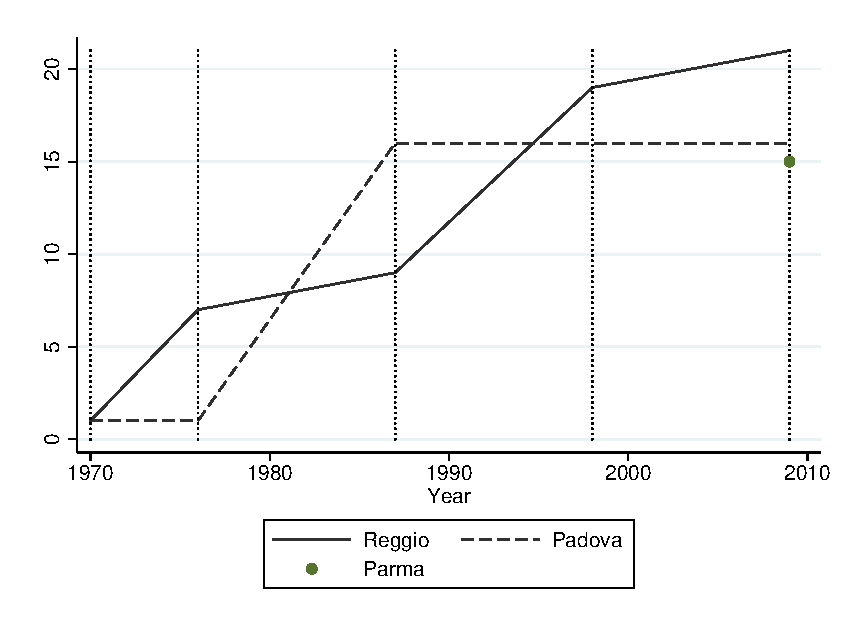
\includegraphics[width=\textwidth]{../../output/image/enroll_per_stat_graph.eps}
            \caption{Percent. of Enrollment in State Preschool}       
        \end{subfigure}
      \begin{subfigure}[ht]{0.48\textwidth}
        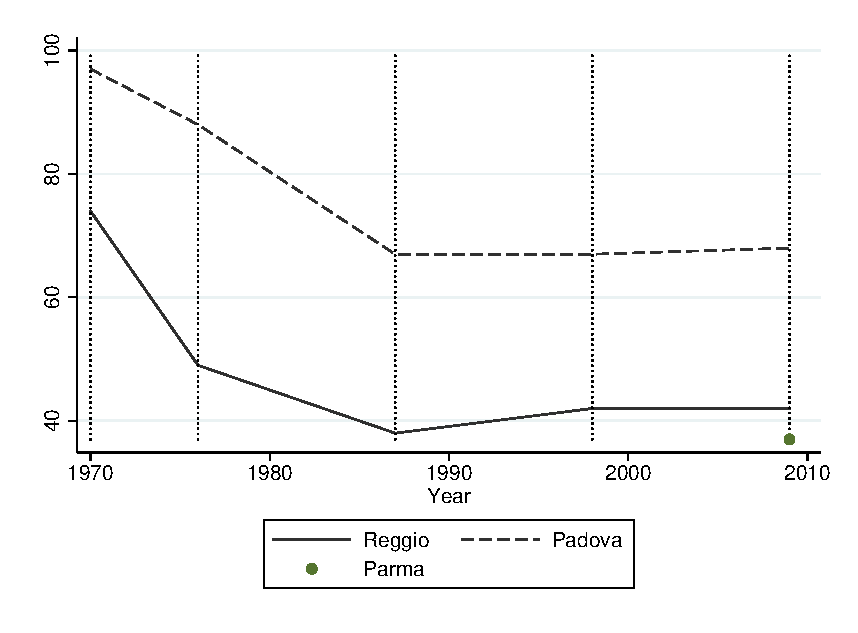
\includegraphics[width=\textwidth]{../../output/image/enroll_per_priv_graph.eps}
        \caption{Percent. of Enrollment in Private Preschool}
        \label{fig:large}
      \end{subfigure}
      \caption{Enrollment Statistics}
    \end{figure}


\subsection{The Survey Data Collection}

The individuals were collected from the population registries in each of the cities in the year ranges of the five cohorts. The sample was then restricted to those individuals living in the same city in which they were raised. All cohorts. except the youngest one, are restricted to individuals who are Italian citizens. In contrast, the youngest cohort includes an oversampling of immigrant children.\footnote{In the adult cohorts there was no immigrant who was preschool age in the same school in which they live. In the adolescent cohort, the number was immigrant born was extremely small.} The sample from Reggio Emilia, across all cohorts, includes an oversampling of those who attended municipal schools, as this is considered the treatment group.

Of the reference sample, 7,109 individuals were randomly selected. Of these, 4,019 completed interviews, resulting in a response rate of 56.5\%. Table~\ref{tab:sample-city-cohort} provides an overview of the birth years for the different cohorts and the counts of the full sample.
\begin{table}[H]
\centering
\begin{threeparttable}
	\caption{Description of the Full Sample by Cohort and City}\label{tab:sample-city-cohort}
	\begin{tabular}{l c c c c c c}
\toprule
Cohort & Birth year(s) & Age at interview & \mc{4}{c}{Count} \\
\cmidrule{4-7}
 & 		&						& Reggio Emilia & Parma & Padova & \textbf{Total} \\
\midrule
\textbf{Children} &  &  &  & &  &  \\ 
\quad Italians & 2006 & 6 & 311 & 291& 278 & 880 \\
\quad Migrants & 2006 & 6 & 110 & 58 & 113 & 281 \\
\textbf{Adolescents} & 1994 & 19 & 300 & 254 & 282 & 836 \\
\textbf{Adults 30s} & 1980-1981 & 32 & 280 & 251 & 251 & 782 \\
\textbf{Adults 40s} & 1969-1970 & 43 & 285 & 254 & 252 & 791 \\
\textbf{Adults 50s} & 1954-1959 & 54-60 & 200 & 103 & 146 & 449 \\
\midrule
\textbf{Total}	& 				& & 1,486 & 1,211 & 1,322 & 4,019 \\
\bottomrule
\end{tabular}
\begin{tablenotes}
\footnotesize
Note: This table presents the number of individuals in the full sample. The age at interview is an approximation given there is some variation in the interview date and birth year within each cohort. In analysis, we combine the Italian and migrant subsamples of the child cohort and control for migrant status.
\end{tablenotes}
\end{threeparttable}
\end{table}

Table~\ref{tab:sample} provides a detailed tabulation of the sample by city, cohort, and school type. It shows that the number of people who do not attend any preschool decreases over time. Whereas the majority of individuals from the age-50 cohort did not attend any preschool, there are few such cases in the child and adolescent cohorts. Table \ref{tab:sample} also shows that the proportion of individual attending municipal preschools is higher in Reggio Emilia than in the other cities.\footnote{This is due to the construction of the sample.} 

\begin{table}[H]
\centering
\scalebox{0.85}{
\begin{threeparttable}
	\caption{Tabulation of Preschool Attendence by Cohort, City, and School Type}\label{tab:sample}
	\begin{tabular}{l*{8}{c}}
\toprule
	&	\mc{7}{c}{Reggio Emilia: 1,486}													\\	\midrule
	&	None	&	Muni	&	State	&	Reli	&	Priv	&	Muni-Affi	&	Other	\\	\midrule
Children	&	2	&	159	&	44	&	92	&	5	&	7	&	1	\\	
Migrants	&	4	&	47	&	38	&	14	&	1	&	3	&	1	\\	
Adolescents	&	7	&	151	&	22	&	98	&	6	&	13	&	0	\\	
Adults 30s	&	57	&	138	&	31	&	40	&	1	&	4	&	8	\\	
Adults 40s	&	80	&	87	&	14	&	52	&	5	&	1	&	43	\\	
Adults 50s	&	147	&	0	&	0	&	29	&	2	&	0	&	20	\\	\midrule
	&	\mc{7}{c}{ Parma: 1,211}													\\	\midrule
	&	None	&	Muni	&	State	&	Reli	&	Priv	&	Muni-Affi	&	Other	\\	\midrule
Children	&	5	&	105	&	42	&	74	&	8	&	52	&	0	\\	
Migrants	&	4	&	25	&	12	&	3	&	6	&	7	&	0	\\	
Adolescents	&	4	&	100	&	52	&	77	&	6	&	5	&	2	\\	
Adults 30s	&	44	&	85	&	56	&	51	&	5	&	4	&	3	\\	
Adults 40s	&	116	&	0	&	0	&	55	&	1	&	4	&	73	\\	
Adults 50s	&	72	&	0	&	0	&	11	&	0	&	10	&	9	\\	\midrule
	&	\mc{7}{c}{Padova: 1,322}													\\	\midrule
	&	None	&	Muni	&	State	&	Reli	&	Priv	&	Muni-Affi	&	Other	\\	\midrule
Children	&	2	&	58	&	45	&	141	&	12	&	19	&	0	\\	
Migrants	&	5	&	33	&	46	&	23	&	1	&	0	&	4	\\	
Adolescents	&	1	&	84	&	46	&	132	&	6	&	7	&	2	\\	
Adults 30s	&	47	&	27	&	27	&	140	&	1	&	7	&	0	\\	
Adults 40s	&	75	&	0	&	0	&	126	&	0	&	10	&	39	\\	
Adults 50s	&	57	&	0	&	0	&	72	&	2	&	6	&	3	\\	

\bottomrule
\end{tabular}


\begin{tablenotes}
Note: This table shows the sample size by city, cohort, and school type. We separate migrants and children for clarity in this table even though they are in the same birth cohort (year of birth: 2006). None: no preschool; Muni.: municipal preschool;  State: state preschool; Relig.: religious preschool; Priv.: private preschool. Muni-Affi: municipal-affiliated preschool; Other: uncategorized preschool.
\end{tablenotes}
\end{threeparttable}
}
\end{table}

The structure of the cohorts allows us to study the effects of the Reggio Approach at different points throughout the life cycle. The children in the youngest cohort were interviewed when they entered primary school, the adolescent cohort when they ended compulsory schooling, and the adult cohorts capture different points of adulthood to measure key outcomes such as engagement in the labor market, health, and family decisions. This cohort structure also allows us to evaluate the Reggio Approach compared to the alternative early childhood experiences over time.

Restricting the sample to individuals living in the same city in which they were raised is necessary because of the municipal structure of the population registries. If the Reggio Approach has a treatment effect on migration out of Reggio Emilia, then our sample might oversample individuals with characteristics that are not predictive of emigration. Although we are not able to quantify the level of emigration, we present the level of immigration into the three cities (Table~\ref{tab:immigration}). For all cohorts, the immigration rates are very similar for all three cities. 

\begin{table}[H]
\centering
\begin{threeparttable}
	\caption{Immigration Rate by City}\label{tab:immigration}
	\begin{table}[ht!]
\caption{\textbf{Percentage of people living in the same city since birth, by cohort}}
\label{tab:SameCity}
\vspace{-5mm}
\begin{center}
\begin{tabular}{ l c c c c }
\hline\hline
\textbf{Cohort} & \textbf{Reggio (\%)} & \textbf{Parma (\%)} & \textbf{Padova (\%)} & \textbf{Total (\%)}\\
\hline
Italian Children born in 2006 (Cohort V)   & 61.3  & 70.2  & 65.1  & 65.2 \\[0.2em]
Adolescents born in 1994 (Cohort IV)       & 58.1  & 63.0  & 64.4  & 61.9 \\[0.2em]
Adults born in 1980-81 (Cohort III)        & 26.5  & 27.5  & 32.6  & 29.0 \\[0.2em]
Adults born in 1969-70 (Cohort II)         & 27.9  & 31.6  & 31.9  & 30.6 \\[0.2em]
Adults born in 1954-59 (Cohort I)          & 28.8  & 27.9  & 31.4  & 29.5 \\[0.2em]
\hline
\textit{Total}         & \textit{32.3\%}  & \textit{32.5\%}  & \textit{35.2\%} & \textit{33.5\%} \\
\hline
\end{tabular}
\end{center}
\footnotesize{{\bfseries Notes:} Reference sample who satisfied the selection criteria (born in the city of residence and of Italian citizenship) as a percentage of the total number of names given by the population registries, broken down by City and Cohort. Source: authors calculations on data provided by the population registries.}
\end{table}

\begin{tablenotes}
\footnotesize
Note: This table presents the immigration rate into the three cities in the years of the three cohorts. These numbers are constructed from the full reference sample.
\end{tablenotes}
\end{threeparttable}
\end{table}

\subsection{The Questionnaire Design}

Separate questionnaires were administered to the children, adolescents, and adults, as well as to the caregivers of the children and adolescents. The questionnaires include items about early childhood experiences, family structure, education, interaction with non-Italians (or with Italians in the case of the migrant children), and measures of cognitive and social-emotional skills. The questionnaires for adults additionally included items about occupation, income, health, and life satisfaction. 


%\subsection{Characteristics of Reggio Emilia, Parma, and Padova}

%Parma and Padova are similar to Reggio Emilia along several characteristics, but have different early childhood education offerings.\footnote{See Section~\ref{sec:eceexperiences} for a discussion of the differences in early childhood education in the three cities. See Appendix~\ref{sec:data-app} for more information on the demographics of the three cities.} All three cities are in Northern Italy; Reggio Emilia and Parma are in the same region of Emilia Romagna, Padova is in the adjacent region of Veneto. 
%Tables~\ref{table:demo-employ} and~\ref{table:demo-other} describe the cities along demographic characteristics. Reggio Emilia and Parma, in addition to being geographically close are socially and economically similar.

%The three cities are similar in employment for different industries, proportion of individuals renting property, and marital status. In 2011, Padova had more individuals with post-secondary degrees compared with Reggio Emilia and Parma. Starting in 1991, the aging index has been higher in Parma than in Reggio Emilia. Starting in 2001, Padova's aging index overtook that of both Reggio Emilia and Parma. A higher aging index indicates there are more individuals over 59 years of age per one hundred individuals under 15 years of age, i.e., an older population with low birth rates. Appendix \ref{sec:data-app} has more detailed information about demographic characteristics of Reggio, Parma, and Padova. 

%\begin{landscape}
%\begin{table}[ht!]
%\begin{center}
%\scriptsize{
%	\caption{Proportion of Individuals in Different Employment and Industry Categories} \label{table:demo-employ}
%	
\begin{tabular}{L{6.5cm} *{3}{*{5}{c} c}}
\hline \\[-7pt]
& \multicolumn{5}{c}{\textbf{Reggio Emilia}} & & \multicolumn{5}{c}{\textbf{Parma}} & & \multicolumn{5}{c}{\textbf{Padova}} \\[3pt]
& \textbf{1971} & \textbf{1981} & \textbf{1991} & \textbf{2001} & \textbf{2011} & & \textbf{1971} & \textbf{1981} & \textbf{1991} & \textbf{2001} & \textbf{2011} & & \textbf{1971} & \textbf{1981} & \textbf{1991} & \textbf{2001} & \textbf{2011} \\[3pt]
\hline \\
\textbf{Employment}\\
\quad Employed (B) & 0.48 & 0.51 & 0.49 & 0.53 & 0.53 & & 0.47 & 0.49 & 0.49 & 0.50 & 0.53 & & 0.45 & 0.46 & 0.45 & 0.47 & 0.49 & \\ 
\quad Employed (F) & 0.28 & 0.37 & 0.38 & 0.43 & 0.46 & & 0.26 & 0.34 & 0.37 & 0.41 & 0.46 & & 0.24 & 0.30 & 0.32 & 0.37 & 0.42 & \\ 
\quad Employed (M) & 0.70 & 0.66 & 0.61 & 0.63 & 0.62 & & 0.70 & 0.66 & 0.62 & 0.60 & 0.60 & & 0.69 & 0.64 & 0.60 & 0.59 & 0.57 & \\[5pt] 
\quad Unemployed (B) & 0.01 & 0.01 & 0.02 & 0.02 & 0.06 & & 0.02 & 0.02 & 0.01 & 0.02 & 0.03 & & 0.02 & 0.01 & 0.02 & 0.03 & 0.04 & \\ 
\quad Unemployed (F) & 0.01 & 0.01 & 0.02 & 0.03 & 0.06 & & 0.01 & 0.02 & 0.01 & 0.02 & 0.03 & & 0.01 & 0.01 & 0.02 & 0.03 & 0.04 & \\ 
\quad Unemployed (M) & 0.02 & 0.01 & 0.02 & 0.02 & 0.05 & & 0.02 & 0.01 & 0.01 & 0.02 & 0.03 & & 0.02 & 0.02 & 0.03 & 0.03 & 0.04 & \\[5pt] 
\quad Homemaker (B) & 0.26 & 0.17 & 0.13 & 0.11 & 0.06 & & 0.28 & 0.20 & 0.16 & 0.12 & 0.07 & & 0.32 & 0.25 & 0.21 & 0.16 & 0.09 & \\ 
\quad Homemaker (F) & 0.50 & 0.33 & 0.25 & 0.20 & 0.11 & & 0.53 & 0.37 & 0.30 & 0.22 & 0.12 & & 0.59 & 0.47 & 0.38 & 0.30 & 0.16 & \\ 
\quad Homemaker (M) & 0.00 & 0.00 & 0.00 & 0.00 & 0.00 & & 0.00 & 0.00 & 0.00 & 0.00 & 0.00 & & 0.00 & 0.00 & 0.00 & 0.00 & 0.01 & \\[5pt] 
\quad Pensioner (B) & 0.15 & 0.21 & 0.23 & 0.24 & 0.25 & & 0.15 & 0.19 & 0.21 & 0.24 & 0.27 & & 0.11 & 0.13 & 0.16 & 0.21 & 0.26 & \\ 
\quad Pensioner (F) & 0.13 & 0.20 & 0.22 & 0.23 & 0.27 & & 0.13 & 0.17 & 0.19 & 0.22 & 0.28 & & 0.07 & 0.09 & 0.12 & 0.18 & 0.27 & \\ 
\quad Pensioner (M) & 0.17 & 0.22 & 0.24 & 0.25 & 0.23 & & 0.18 & 0.21 & 0.23 & 0.26 & 0.25 & & 0.15 & 0.17 & 0.20 & 0.26 & 0.25 & \\[5pt] 
\quad Student (B) & 0.07 & 0.07 & 0.08 & 0.06 & 0.06 & & 0.07 & 0.08 & 0.09 & 0.07 & 0.07 & & 0.09 & 0.11 & 0.11 & 0.08 & 0.08 & \\ 
\quad Student (F) & 0.06 & 0.07 & 0.08 & 0.05 & 0.06 & & 0.06 & 0.08 & 0.08 & 0.06 & 0.06 & & 0.07 & 0.10 & 0.10 & 0.07 & 0.07 & \\ 
\quad Student (M) & 0.08 & 0.08 & 0.08 & 0.06 & 0.07 & & 0.08 & 0.09 & 0.09 & 0.07 & 0.07 & & 0.11 & 0.13 & 0.12 & 0.08 & 0.08 & \\[5pt] 
\quad Other (B) & 0.03 & 0.03 & 0.05 & 0.05 & 0.04 & & 0.02 & 0.02 & 0.04 & 0.05 & 0.04 & & 0.02 & 0.03 & 0.05 & 0.05 & 0.05 & \\ 
\quad Other (F) & 0.03 & 0.02 & 0.05 & 0.05 & 0.04 & & 0.02 & 0.02 & 0.04 & 0.05 & 0.04 & & 0.02 & 0.02 & 0.05 & 0.05 & 0.04 & \\ 
\quad Other (M) & 0.04 & 0.03 & 0.04 & 0.04 & 0.04 & & 0.02 & 0.03 & 0.04 & 0.05 & 0.04 & & 0.03 & 0.04 & 0.05 & 0.05 & 0.05 & \\[5pt] 
\textbf{Industry}\\
\quad Agriculture, Forestry And Fishing (B) &   . & 0.08 & 0.04 & 0.04 & 0.04 & &   . & 0.05 & 0.02 & 0.02 & 0.03 & &   . & 0.01 & 0.01 & 0.01 & 0.01 & \\ 
\quad Agriculture, Forestry And Fishing (F) &   . & 0.06 & 0.03 & 0.03 & 0.02 & &   . & 0.04 & 0.01 & 0.02 & 0.02 & &   . & 0.01 & 0.01 & 0.01 & 0.01 & \\ 
\quad Agriculture, Forestry And Fishing (M) &   . & 0.10 & 0.05 & 0.04 & 0.05 & &   . & 0.05 & 0.03 & 0.03 & 0.04 & &   . & 0.02 & 0.01 & 0.01 & 0.02 & \\[5pt] 
\quad Finance, Professional, Scientific, Admin (B) &   . & 0.07 & 0.11 & 0.11 & 0.14 & &   . & 0.08 & 0.13 & 0.14 & 0.17 & &   . & 0.09 & 0.15 & 0.17 & 0.19 & \\ 
\quad Finance, Professional, Scientific, Admin (F) &   . & 0.06 & 0.12 & 0.12 & 0.15 & &   . & 0.07 & 0.15 & 0.14 & 0.18 & &   . & 0.08 & 0.15 & 0.17 & 0.19 & \\ 
\quad Finance, Professional, Scientific, Admin (M) &   . & 0.07 & 0.10 & 0.11 & 0.13 & &   . & 0.08 & 0.12 & 0.13 & 0.16 & &   . & 0.09 & 0.15 & 0.17 & 0.20 & \\[5pt] 
\quad Trade, Hotels And Restaurants  (B) &   . & 0.19 & 0.20 & 0.19 & 0.18 & &   . & 0.20 & 0.19 & 0.18 & 0.17 & &   . & 0.26 & 0.23 & 0.20 & 0.16 & \\ 
\quad Trade, Hotels And Restaurants  (F) &   . & 0.20 & 0.21 & 0.21 & 0.20 & &   . & 0.21 & 0.21 & 0.20 & 0.18 & &   . & 0.24 & 0.21 & 0.19 & 0.16 & \\ 
\quad Trade, Hotels And Restaurants  (M) &   . & 0.18 & 0.19 & 0.18 & 0.16 & &   . & 0.19 & 0.18 & 0.17 & 0.15 & &   . & 0.26 & 0.23 & 0.20 & 0.17 & \\[5pt] 
\quad Transport, Storage, Info, Communication  (B) &   . & 0.05 & 0.04 & 0.04 & 0.06 & &   . & 0.05 & 0.05 & 0.04 & 0.06 & &   . & 0.06 & 0.05 & 0.05 & 0.07 & \\ 
\quad Transport, Storage, Info, Communication  (F) &   . & 0.02 & 0.03 & 0.02 & 0.03 & &   . & 0.02 & 0.03 & 0.02 & 0.04 & &   . & 0.03 & 0.03 & 0.03 & 0.04 & \\ 
\quad Transport, Storage, Info, Communication  (M) &   . & 0.06 & 0.05 & 0.05 & 0.07 & &   . & 0.07 & 0.06 & 0.05 & 0.08 & &   . & 0.08 & 0.07 & 0.06 & 0.09 & \\[5pt] 
\quad Other Activities  (B) &   . & 0.24 & 0.23 & 0.25 & 0.28 & &   . & 0.25 & 0.25 & 0.28 & 0.31 & &   . & 0.32 & 0.32 & 0.35 & 0.37 & \\ 
\quad Other Activities  (F) &   . & 0.36 & 0.34 & 0.38 & 0.43 & &   . & 0.39 & 0.36 & 0.41 & 0.44 & &   . & 0.47 & 0.44 & 0.47 & 0.51 & \\ 
\quad Other Activities  (M) &   . & 0.16 & 0.16 & 0.15 & 0.15 & &   . & 0.17 & 0.18 & 0.19 & 0.20 & &   . & 0.24 & 0.25 & 0.27 & 0.25 & \\[5pt] 
\hline \\[-7pt]
\multicolumn{19}{L{24cm}}{\textbf{Note:} This table presents the percentage of individuals in different employment and industry categories within each city during each of the 5 listed years. Percentages are reported for females (F), males (M), and both genders (B) combined. The percentages are calculated using the total number of individuals above age 15 for the denominator. Data were collected from ISTAT and regional agencies.}
\end{tabular}

%}
%\end{center}
%\end{table}
%\end{landscape}

%\begin{landscape}
%\begin{table}[ht!]
%\begin{center}
%\scriptsize{
%	\caption{Proportion of Individuals in Different Education, Rental, and Marital Categories} \label{table:demo-other}
%	
\begin{tabular}{L{5cm} *{3}{*{5}{c} c}}
\hline \\[-7pt]
& \multicolumn{5}{c}{\textbf{Reggio Emilia}} & & \multicolumn{5}{c}{\textbf{Parma}} & & \multicolumn{5}{c}{\textbf{Padova}} \\[3pt]
& \textbf{1971} & \textbf{1981} & \textbf{1991} & \textbf{2001} & \textbf{2011} & & \textbf{1971} & \textbf{1981} & \textbf{1991} & \textbf{2001} & \textbf{2011} & & \textbf{1971} & \textbf{1981} & \textbf{1991} & \textbf{2001} & \textbf{2011} \\[3pt]
\hline \\
~\\[-4pt]
\textbf{Education}\\
\quad $<$ Primary (B) & 0.27 & 0.15 & 0.10 & 0.08 & 0.07 & & 0.28 & 0.14 & 0.09 & 0.07 & 0.06 & & 0.23 & 0.13 & 0.08 & 0.06 & 0.06 & \\ 
\quad $<$ Primary (F) & 0.31 & 0.17 & 0.11 & 0.09 & 0.08 & & 0.32 & 0.16 & 0.10 & 0.08 & 0.07 & & 0.26 & 0.14 & 0.09 & 0.07 & 0.06 & \\ 
\quad $<$ Primary (M) & 0.23 & 0.13 & 0.08 & 0.07 & 0.07 & & 0.23 & 0.12 & 0.07 & 0.06 & 0.06 & & 0.20 & 0.11 & 0.06 & 0.06 & 0.06 & \\[5pt] 
\quad Primary (B) & 0.45 & 0.43 & 0.34 & 0.26 & 0.18 & & 0.43 & 0.41 & 0.32 & 0.24 & 0.18 & & 0.41 & 0.35 & 0.27 & 0.21 & 0.17 & \\ 
\quad Primary (F) & 0.44 & 0.45 & 0.37 & 0.28 & 0.21 & & 0.42 & 0.43 & 0.35 & 0.27 & 0.20 & & 0.42 & 0.39 & 0.31 & 0.25 & 0.20 & \\ 
\quad Primary (M) & 0.46 & 0.40 & 0.31 & 0.22 & 0.16 & & 0.43 & 0.38 & 0.28 & 0.21 & 0.15 & & 0.39 & 0.31 & 0.22 & 0.17 & 0.13 & \\[5pt] 
\quad Lower Secondary (B) & 0.16 & 0.24 & 0.27 & 0.27 & 0.27 & & 0.16 & 0.24 & 0.28 & 0.25 & 0.25 & & 0.20 & 0.26 & 0.28 & 0.25 & 0.23 & \\ 
\quad Lower Secondary (F) & 0.14 & 0.21 & 0.23 & 0.23 & 0.24 & & 0.15 & 0.21 & 0.25 & 0.23 & 0.22 & & 0.19 & 0.24 & 0.26 & 0.23 & 0.21 & \\ 
\quad Lower Secondary (M) & 0.17 & 0.26 & 0.31 & 0.31 & 0.31 & & 0.18 & 0.26 & 0.31 & 0.28 & 0.27 & & 0.22 & 0.28 & 0.31 & 0.27 & 0.24 & \\[5pt] 
\quad High School (B) & 0.10 & 0.15 & 0.24 & 0.30 & 0.33 & & 0.10 & 0.16 & 0.24 & 0.30 & 0.32 & & 0.12 & 0.19 & 0.27 & 0.30 & 0.31 & \\ 
\quad High School (F) & 0.09 & 0.14 & 0.24 & 0.29 & 0.33 & & 0.09 & 0.16 & 0.24 & 0.29 & 0.31 & & 0.10 & 0.17 & 0.25 & 0.29 & 0.30 & \\ 
\quad High School (M) & 0.11 & 0.16 & 0.24 & 0.30 & 0.33 & & 0.11 & 0.17 & 0.25 & 0.31 & 0.33 & & 0.13 & 0.20 & 0.28 & 0.32 & 0.33 & \\[5pt] 
\quad Post Secondary Degree (B) & 0.02 & 0.04 & 0.06 & 0.10 & 0.14 & & 0.03 & 0.05 & 0.07 & 0.14 & 0.19 & & 0.04 & 0.07 & 0.11 & 0.17 & 0.24 & \\ 
\quad Post Secondary Degree (F) & 0.02 & 0.03 & 0.05 & 0.10 & 0.15 & & 0.02 & 0.04 & 0.06 & 0.13 & 0.20 & & 0.03 & 0.05 & 0.09 & 0.16 & 0.23 & \\ 
\quad Post Secondary Degree (M) & 0.03 & 0.05 & 0.07 & 0.10 & 0.13 & & 0.04 & 0.06 & 0.09 & 0.14 & 0.19 & & 0.06 & 0.09 & 0.13 & 0.19 & 0.24 & \\[5pt] 
~\\[-4pt]
\textbf{Rental Status}\\
%\quad Other (B) & 0.05 & 0.06 & 0.07 & 0.08 & 0.09 & & 0.05 & 0.05 & 0.06 & 0.08 & 0.08 & & 0.04 & 0.04 & 0.05 & 0.06 & 0.08 & \\ 
%\quad Owned (B) & 0.41 & 0.53 & 0.63 & 0.68 & 0.67 & & 0.34 & 0.46 & 0.58 & 0.66 & 0.67 & & 0.39 & 0.47 & 0.62 & 0.69 & 0.70 & \\ 
\quad Rented (B) & 0.53 & 0.41 & 0.30 & 0.23 & 0.23 & & 0.61 & 0.49 & 0.35 & 0.26 & 0.25 & & 0.58 & 0.49 & 0.33 & 0.25 & 0.23 & \\ 
~\\[-4pt]
\textbf{Marital Status}\\
\quad Divorced (B) &   . & 0.02 & 0.02 & 0.04 & 0.06 & &   . & 0.02 & 0.03 & 0.04 & 0.06 & &   . & 0.02 & 0.03 & 0.04 & 0.06 & \\ 
\quad Married (B) & 0.52 & 0.52 & 0.51 & 0.49 & 0.44 & & 0.53 & 0.53 & 0.52 & 0.50 & 0.43 & & 0.48 & 0.48 & 0.48 & 0.47 & 0.43 & \\ 
\quad Never Married (B) & 0.40 & 0.37 & 0.37 & 0.38 & 0.42 & & 0.39 & 0.37 & 0.36 & 0.37 & 0.41 & & 0.46 & 0.43 & 0.41 & 0.40 & 0.41 & \\ 
\quad Widowed (B) & 0.08 & 0.09 & 0.09 & 0.09 & 0.08 & & 0.08 & 0.09 & 0.10 & 0.10 & 0.09 & & 0.07 & 0.07 & 0.09 & 0.09 & 0.09 & \\ 
~\\[-4pt]
\textbf{Population Metrics}\\
\quad Aging Index (B) & 69.49 & 101.51 & 171.58 & 155.22 & 131.09 & & 63.32 & 99.35 & 192.66 & 210.50 & 184.46 & & 44.27 & 73.08 & 160.67 & 202.58 & 205.18 & \\ 
\quad Dependency Ratio (B) & 46.34 & 41.05 & 46.98 & 51.69 & 54.17 & & 47.05 & 47.92 & 43.79 & 50.36 & 56.70 & & 51.97 & 45.65 & 40.58 & 50.29 & 59.41 & \\ 
%\quad Eatio (B) & 1.68 & 3.22 & 4.51 & 3.55 & 3.11 & & 1.51 & 3.34 & 5.24 & 5.00 & 4.35 & & 1.08 & 2.50 & 4.25 & 4.93 & 5.02 & \\ 
\hline \\[-7pt]
\multicolumn{19}{L{24cm}}{\textbf{Note:} This table presents the percentage of individuals in different education, rental and marital categories within each city during each of the 5 listed years. Percentages are reported for females (F), males (M), and both genders (B) combined. The percentages are calculated using the total number of individuals above age 15 for the denominator. Data were collected from ISTAT and regional agencies. Aging Index: number of people older than 59 years old per one hundred people younger than 15 years; Dependency Ratio: number of people older than 64 or younger than 15 divided by the number of people between 15 and 64 years old.}
\end{tabular}


%}
%\end{center}
%\end{table}
%\end{landscape}




